\documentclass{ximera}

\author{Anna Davis} \title{MTH 140 Homework 1} 

\begin{document}

\begin{abstract}

\end{abstract}
\maketitle
 \textit{Certificate due: 8/24/2020 at 11:59 p.m.}
\begin{problem}\label{prob:140hom1prob1}
Classify each variable.
\begin{enumerate}
    \item Heart rate (beats per minute).  \wordChoice{\choice{qualitative}, \choice[correct]{quantitative discrete},\choice{quantitative continuous}}
    \item  Weight.  \wordChoice{\choice{qualitative}, \choice{quantitative discrete},\choice[correct]{quantitative continuous}} 
    \item  Number of points an NBA team scores in a game. \wordChoice{\choice{qualitative}, \choice[correct]{quantitative discrete},\choice[correct]{quantitative continuous}}
    \item  The AVERAGE number of points per game an NBA team scores in a season. \wordChoice{\choice{qualitative}, \choice{quantitative discrete},\choice[correct]{quantitative continuous}} 
    \item Name of a team. \wordChoice{\choice[correct]{qualitative}, \choice{quantitative discrete},\choice{quantitative continuous}}
    \item Height.  \wordChoice{\choice{qualitative}, \choice{quantitative discrete},\choice[correct]{quantitative continuous}} 
    \item Price of gasoline.  \wordChoice{\choice{qualitative}, \choice{quantitative discrete},\choice[correct]{quantitative continuous}} 
    \item Credit card balance.  \wordChoice{\choice{qualitative}, \choice{quantitative discrete},\choice[correct]{quantitative continuous}} 
    \item Number of pets a person has.  \wordChoice{\choice{qualitative}, \choice[correct]{quantitative discrete},\choice{quantitative continuous}} 
    \item Dog breed. \wordChoice{\choice[correct]{qualitative}, \choice{quantitative discrete},\choice{quantitative continuous}}
\end{enumerate}
\end{problem}

\begin{problem}\label{prob:140hom1prob2}
Each schematic below corresponds to a sampling method.  Identify the sampling method.
\begin{enumerate}
    \item Sampling Method: \wordChoice{\choice{Systematic}, \choice{Cluster},\choice[correct]{Stratified}}
    \begin{image}
   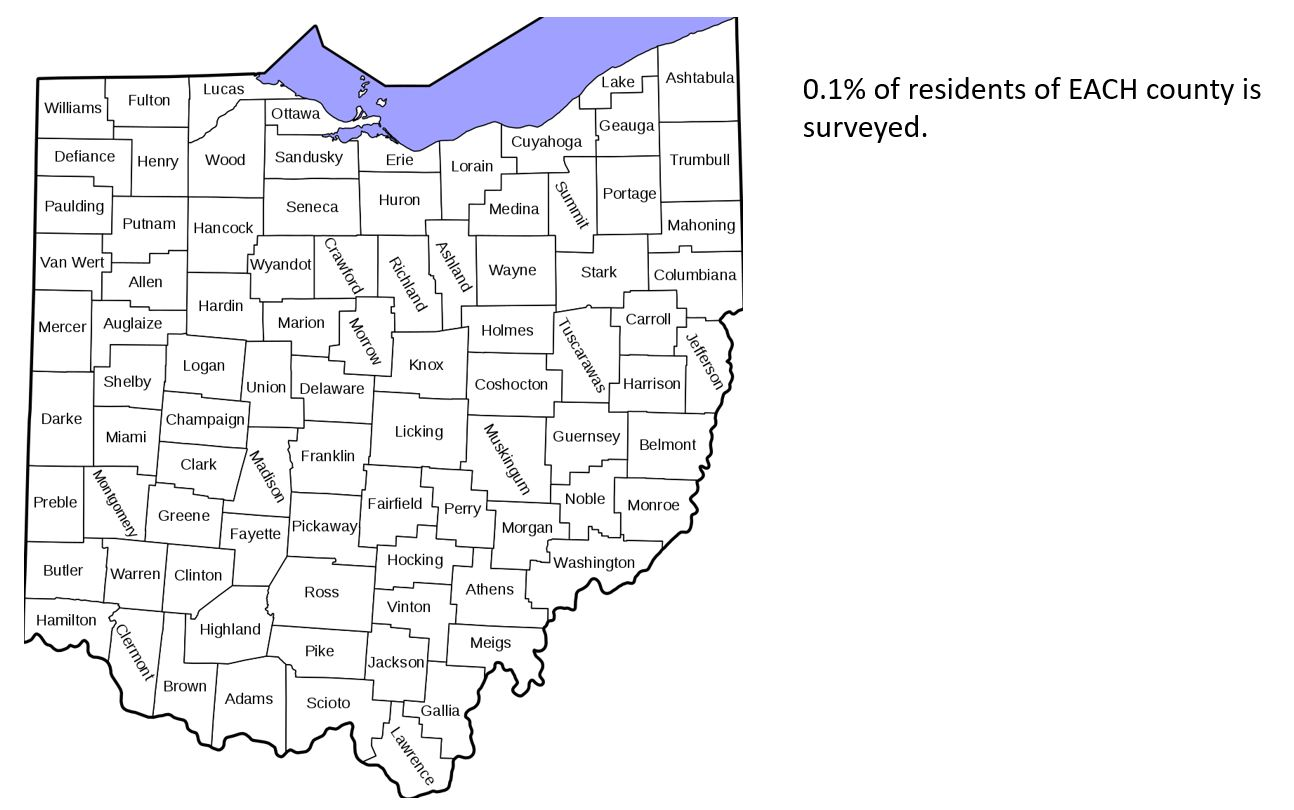
\includegraphics[height=1in]{140H1pic3.jpg}
 \end{image}
 \item Sampling Method: \wordChoice{\choice[correct]{Systematic}, \choice{Cluster},\choice{Stratified}}
    \begin{image}
   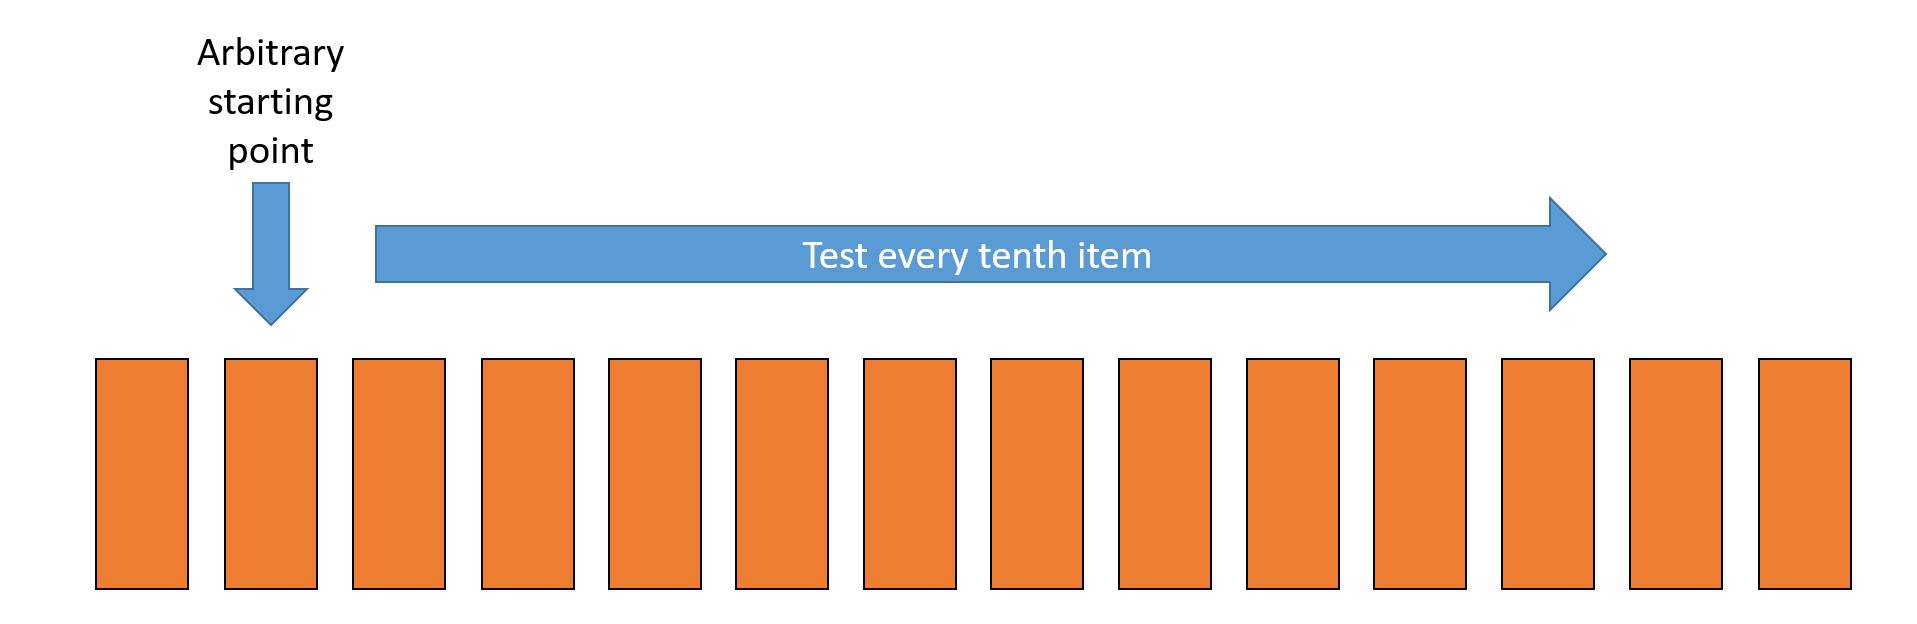
\includegraphics[height=1in]{140H1pic1.jpg}
 \end{image}
 \item Sampling Method: \wordChoice{\choice{Systematic}, \choice[correct]{Cluster},\choice{Stratified}}
    \begin{image}
   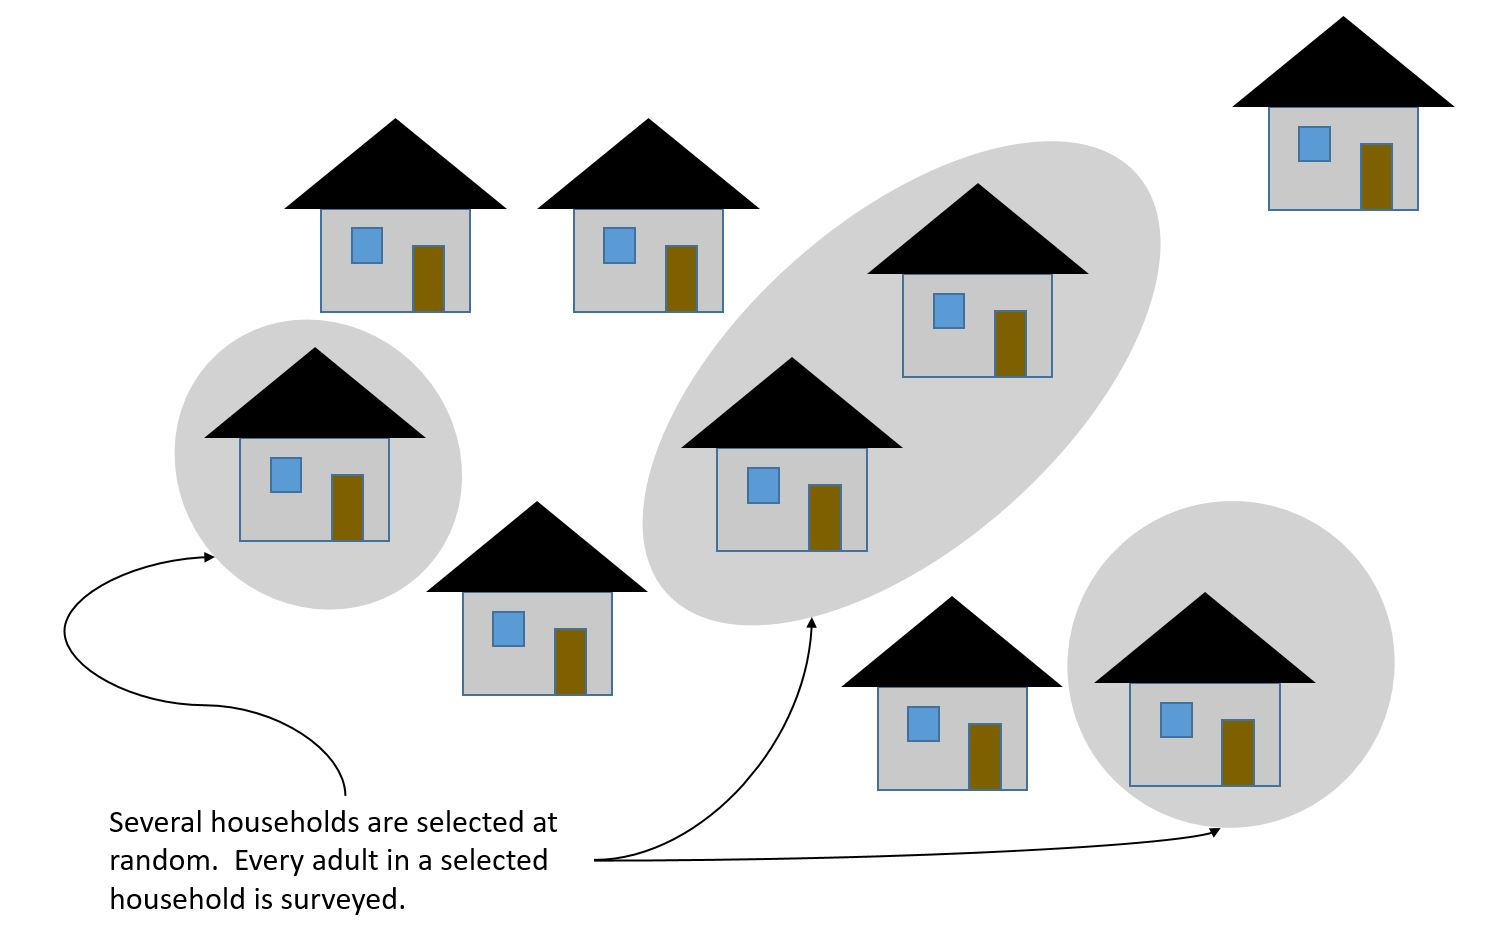
\includegraphics[height=1in]{140H1pic2.jpg}
 \end{image}
\end{enumerate}
\end{problem}

\begin{problem}\label{prob:140hom1prob3}
Classify each scenario according to the sampling method.
\begin{enumerate}
    \item A school principal wants to know how parents feel about a certain issue.  He asks a question about the issue of all parents passing by the front door of the school as they drop off their kids.
    \begin{multipleChoice}  
\choice{Simple Random Sample}  
\choice{Systematic}  
\choice{Cluster}  
\choice{Stratified}  
\choice[correct]{Sample of Convenience} 
\end{multipleChoice}  

 \item A gym wants to know how its members feel about group fitness classes.  The gym manager randomly selects 100 members from the membership list and asks them for their opinion.
    \begin{multipleChoice}  
\choice[correct]{Simple Random Sample}  
\choice{Systematic}  
\choice{Cluster}  
\choice{Stratified}  
\choice{Sample of Convenience} 
\end{multipleChoice}  

\item An executive at a large company wants to know how much time an employee spends on safety training.  The executive polls 20\% of employees at each of the company's cites.
    \begin{multipleChoice}  
\choice{Simple Random Sample}  
\choice{Systematic}  
\choice{Cluster}  
\choice[correct]{Stratified}  
\choice{Sample of Convenience} 
\end{multipleChoice}  

\item A tour company wants to survey its customers.  The tour company selects 10 of its 150 tour buses at random and administers a survey to all passengers on each of the 10 buses.
    \begin{multipleChoice}  
\choice{Simple Random Sample}  
\choice{Systematic}  
\choice[correct]{Cluster}  
\choice{Stratified}  
\choice{Sample of Convenience} 
\end{multipleChoice}  
\end{enumerate}
\end{problem}
\end{document} 